\documentclass[letterpaper]{article}
\usepackage[utf8]{inputenc}
\usepackage[margin=1in]{geometry} 

\author{Trevor Klar}
\title{}

%% Useful packages
\usepackage{amssymb, amsmath, amsthm} 
%\usepackage{graphicx}  %%this is currently enabled in the default document, so it is commented out here. 
\usepackage{calrsfs}
\usepackage{braket}
\usepackage{mathtools}
\usepackage{lipsum}
\usepackage{tikz}
\usetikzlibrary{cd}
\usepackage{verbatim}
%\usepackage{ntheorem}% for theorem-like environments
\usepackage{mdframed}%can make highlighted boxes of text
%Use case: https://tex.stackexchange.com/questions/46828/how-to-highlight-important-parts-with-a-gray-background
\usepackage{wrapfig}
\usepackage{centernot}
\usepackage{subcaption}%\begin{subfigure}{0.5\textwidth}
\usepackage{pgfplots}
\pgfplotsset{compat=1.13}
\usepackage[colorinlistoftodos]{todonotes}
\usepackage[colorlinks=true, allcolors=blue]{hyperref}
\usepackage{xfrac}					%to make slanted fractions \sfrac{numerator}{denominator}
\usepackage{enumitem}            
    %syntax: \begin{enumerate}[label=(\alph*)]
    %possible arguments: f \alph*, \Alph*, \arabic*, \roman* and \Roman*
\usetikzlibrary{arrows,shapes.geometric,fit}

\DeclareMathAlphabet{\pazocal}{OMS}{zplm}{m}{n}
%% Use \pazocal{letter} to typeset a letter in the other kind 
%%  of math calligraphic font. 

%% This puts the QED block at the end of each proof, the way I like it. 
\renewenvironment{proof}{{\bfseries Proof}}{\qed}
\makeatletter
\renewenvironment{proof}[1][\bfseries \proofname]{\par
  \pushQED{\qed}%
  \normalfont \topsep6\p@\@plus6\p@\relax
  \trivlist
  %\itemindent\normalparindent
  \item[\hskip\labelsep
        \scshape
    #1\@addpunct{}]\ignorespaces
}{%
  \popQED\endtrivlist\@endpefalse
}
\makeatother

%% This adds a \rewnewtheorem command, which enables me to override the settings for theorems contained in this document.
\makeatletter
\def\renewtheorem#1{%
  \expandafter\let\csname#1\endcsname\relax
  \expandafter\let\csname c@#1\endcsname\relax
  \gdef\renewtheorem@envname{#1}
  \renewtheorem@secpar
}
\def\renewtheorem@secpar{\@ifnextchar[{\renewtheorem@numberedlike}{\renewtheorem@nonumberedlike}}
\def\renewtheorem@numberedlike[#1]#2{\newtheorem{\renewtheorem@envname}[#1]{#2}}
\def\renewtheorem@nonumberedlike#1{  
\def\renewtheorem@caption{#1}
\edef\renewtheorem@nowithin{\noexpand\newtheorem{\renewtheorem@envname}{\renewtheorem@caption}}
\renewtheorem@thirdpar
}
\def\renewtheorem@thirdpar{\@ifnextchar[{\renewtheorem@within}{\renewtheorem@nowithin}}
\def\renewtheorem@within[#1]{\renewtheorem@nowithin[#1]}
\makeatother

%% This makes theorems and definitions with names show up in bold, the way I like it. 
\makeatletter
\def\th@plain{%
  \thm@notefont{}% same as heading font
  \itshape % body font
}
\def\th@definition{%
  \thm@notefont{}% same as heading font
  \normalfont % body font
}
\makeatother

%===============================================
%==============Shortcut Commands================
%===============================================
\newcommand{\ds}{\displaystyle}
\newcommand{\B}{\mathcal{B}}
\newcommand{\C}{\mathbb{C}}
\newcommand{\F}{\mathbb{F}}
\newcommand{\N}{\mathbb{N}}
\newcommand{\R}{\mathbb{R}}
\newcommand{\Q}{\mathbb{Q}}
\newcommand{\T}{\mathcal{T}}
\newcommand{\Z}{\mathbb{Z}}
\renewcommand\qedsymbol{$\blacksquare$}
\newcommand{\qedwhite}{\hfill\ensuremath{\square}}
\newcommand*\conj[1]{\overline{#1}}
\newcommand*\closure[1]{\overline{#1}}
\newcommand*\mean[1]{\overline{#1}}
%\newcommand{\inner}[1]{\left< #1 \right>}
\newcommand{\inner}[2]{\left< #1, #2 \right>}
\newcommand{\powerset}[1]{\pazocal{P}(#1)}
%% Use \pazocal{letter} to typeset a letter in the other kind 
%%  of math calligraphic font. 
\newcommand{\cardinality}[1]{\left| #1 \right|}
\newcommand{\domain}[1]{\mathcal{D}(#1)}
\newcommand{\image}{\text{Im}}
\newcommand{\inv}[1]{#1^{-1}}
\newcommand{\preimage}[2]{#1^{-1}\left(#2\right)}
\newcommand{\script}[1]{\mathcal{#1}}


\newenvironment{highlight}{\begin{mdframed}[backgroundcolor=gray!20]}{\end{mdframed}}

\DeclarePairedDelimiter\ceil{\lceil}{\rceil}
\DeclarePairedDelimiter\floor{\lfloor}{\rfloor}

%===============================================
%===============My Tikz Commands================
%===============================================
\newcommand{\drawsquiggle}[1]{\draw[shift={(#1,0)}] (.005,.05) -- (-.005,.02) -- (.005,-.02) -- (-.005,-.05);}
\newcommand{\drawpoint}[2]{\draw[*-*] (#1,0.01) node[below, shift={(0,-.2)}] {#2};}
\newcommand{\drawopoint}[2]{\draw[o-o] (#1,0.01) node[below, shift={(0,-.2)}] {#2};}
\newcommand{\drawlpoint}[2]{\draw (#1,0.02) -- (#1,-0.02) node[below] {#2};}
\newcommand{\drawlbrack}[2]{\draw (#1+.01,0.02) --(#1,0.02) -- (#1,-0.02) -- (#1+.01,-0.02) node[below, shift={(-.01,0)}] {#2};}
\newcommand{\drawrbrack}[2]{\draw (#1-.01,0.02) --(#1,0.02) -- (#1,-0.02) -- (#1-.01,-0.02) node[below, shift={(+.01,0)}] {#2};}

%***********************************************
%**************Start of Document****************
%***********************************************

%===============================================
%===============Theorem Styles==================
%===============================================

%================Default Style==================
\theoremstyle{plain}% is the default. it sets the text in italic and adds extra space above and below the \newtheorems listed below it in the input. it is recommended for theorems, corollaries, lemmas, propositions, conjectures, criteria, and (possibly; depends on the subject area) algorithms.
\newtheorem{theorem}{Theorem}
\numberwithin{theorem}{section} %This sets the numbering system for theorems to number them down to the {argument} level. I have it set to number down to the {section} level right now.
\newtheorem*{theorem*}{Theorem} %Theorem with no numbering
\newtheorem{corollary}[theorem]{Corollary}
\newtheorem*{corollary*}{Corollary}
\newtheorem{conjecture}[theorem]{Conjecture}
\newtheorem{lemma}[theorem]{Lemma}
\newtheorem*{lemma*}{Lemma}
\newtheorem{proposition}[theorem]{Proposition}
\newtheorem*{proposition*}{Proposition}
\newtheorem{problemstatement}[theorem]{Problem Statement}


%==============Definition Style=================
\theoremstyle{definition}% adds extra space above and below, but sets the text in roman. it is recommended for definitions, conditions, problems, and examples; i've alse seen it used for exercises.
\newtheorem{definition}[theorem]{Definition}
\newtheorem*{definition*}{Definition}
\newtheorem{condition}[theorem]{Condition}
\newtheorem{problem}[theorem]{Problem}
\newtheorem{example}[theorem]{Example}
\newtheorem*{example*}{Example}
\newtheorem*{counterexample*}{Counterexample}
\newtheorem*{romantheorem*}{Theorem} %Theorem with no numbering
\newtheorem{exercise}{Exercise}
\numberwithin{exercise}{section}
\newtheorem{algorithm}[theorem]{Algorithm}

%================Remark Style===================
\theoremstyle{remark}% is set in roman, with no additional space above or below. it is recommended for remarks, notes, notation, claims, summaries, acknowledgments, cases, and conclusions.
\newtheorem{remark}[theorem]{Remark}
\newtheorem*{remark*}{Remark}
\newtheorem{notation}[theorem]{Notation}
\newtheorem*{notation*}{Notation}
%\newtheorem{claim}[theorem]{Claim}  %%use this if you ever want claims to be numbered
\newtheorem*{claim}{Claim}



\begin{document}
\maketitle

\begin{theorem*}
Let $S$ be a bounded set of real numbers. If $S$ is uncountably infinite, then it has an infinite number of limit points. 
\end{theorem*}

\begin{proof}
To prove this theorem, we will prove the contrapositive. That is, we will show that if $S$ has a finite number of limit points, then it is countable. 

Suppose $S$ has a finite number of limit points. Let $L = \{ L_1, L_2, L_3, \, \ldots \, L_N \}$ be the set of limit points of $S$. Since it is given that $S$ is bounded, let $b_0 = \inf(S)$ and let $b_N = \sup(S)$, and place $\{b_n\}_{n=1}^{N-1}$ such that $L_n < b_n < L_{n+1} $ as shown.

\begin{center}
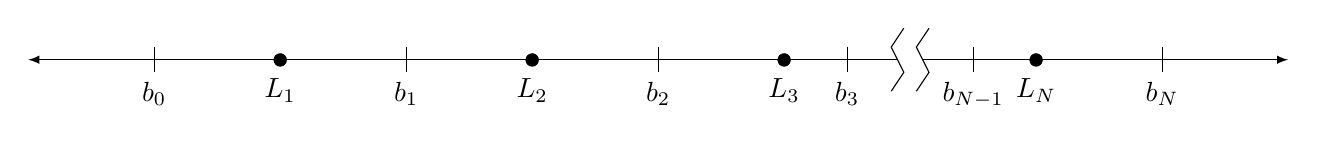
\begin{tikzpicture}[xscale=16, yscale=8]

\draw [latex-] (0,0) -- (.7-.01,0);
\draw [-latex] (.7+.01,0) -- (1,0);

\drawsquiggle{.7-.01}
\drawsquiggle{.7+.01}

\foreach \n in {1,2,3}
  {\drawpoint{\n/5}{$L_{\n}$}}
\drawpoint{4/5}{$L_N$}

\drawlpoint{1/10}{$b_0$}
\drawlpoint{3/10}{$b_1$}
\drawlpoint{5/10}{$b_2$}
\drawlpoint{3/5+1/20}{$b_3$}
\drawlpoint{4/5-1/20}{$b_{N-1}$}
\drawlpoint{9/10}{$b_N$}

\end{tikzpicture}
\end{center}
%
Consider the region $[b_0, b_1]$. Since $L_1$ is the only limit point of $S$ in this region; then for any $\epsilon>0$ the subset $[b_0,b_1] \setminus [L_1 - \epsilon, L_1 + \epsilon]$ contains finitely many elements of $S$. 

\begin{center}
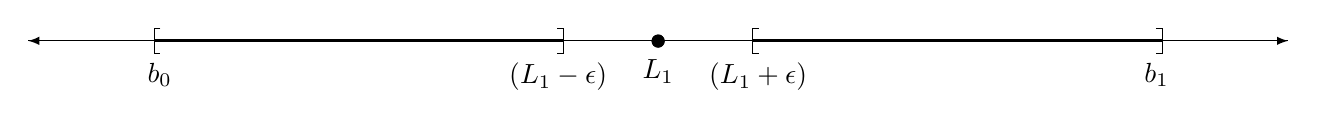
\begin{tikzpicture}[xscale=8, yscale=8]

\draw [latex-] (-1,0) -- (1,0);
\draw [-latex] (-1,0) -- (1,0);

\drawpoint{0}{$L_1$}

\drawlbrack{-.8}{$b_0$}
\draw [very thick] (-.8,0) -- (-.15,0);
\drawrbrack{-.15}{$(L_1-\epsilon)$}

\drawlbrack{.15}{$(L_1+\epsilon)$}
\draw [very thick] (.8,0) -- (.15,0);
\drawrbrack{.8}{$b_1$}

\end{tikzpicture}
\end{center}
%
This is because if not, then $[b_0,b_1] \setminus [L_1 - \epsilon, L_1 + \epsilon])$ would be bounded and infinite, so it would contain a limit point by the Bolzano-Weierstrauss Theorem. 
%
Now, we will proceed to count the elements of $S$ in $[b_0, b_1]$. 

Let $\epsilon_1 = \dfrac{1}{2} \min(|b_0-L|, |b_1-L|)$.

Let $\epsilon_2 = \dfrac{1}{2} \epsilon_1 \quad$

Let $\epsilon_n = \dfrac{1}{2} \epsilon_{n-1} \quad$

\begin{center}
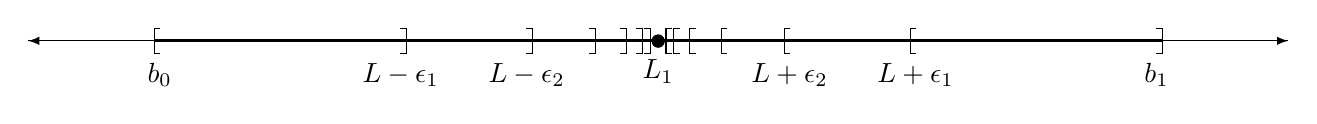
\begin{tikzpicture}[xscale=8, yscale=8]

\draw [latex-] (-1,0) -- (1,0);
\draw [-latex] (-1,0) -- (1,0);

\drawpoint{0}{$L_1$}

\drawlbrack{-.8}{$b_0$}
\draw [very thick] (-.8,0) -- (.8,0);
\drawrbrack{.8}{$b_1$}

\foreach \n in {1,2}
  {\drawrbrack{-.8/2^\n}{$L-\epsilon_{\n}$}}
\foreach \n in {3,4,...,6}
  {\drawrbrack{-.8/2^\n}{}}
  
\foreach \n in {1,2}
  {\drawlbrack{.8/2^\n}{$L+\epsilon_{\n}$}}
\foreach \n in {3,4,...,6}
  {\drawlbrack{.8/2^\n}{}}

%\drawrbrack{-.4}{$(L_1-\epsilon)$}

%\drawlbrack{.15}{$(L_1+\epsilon)$}
%\draw [very thick] (.8,0) -- (.15,0);


\end{tikzpicture}
\end{center}
%
According to the reasoning above, each of the following sets has a finite number of elements:

$A_1 = S \cap ( [b_0,b_1] \setminus [L_1 - \epsilon_1, L_1 + \epsilon_1] )$

$A_2 = S \cap ( [L_1 - \epsilon_1, L_1 + \epsilon_1] \setminus [L_1 - \epsilon_2, L_1 + \epsilon_2] )$

$A_3 = S \cap ( [L_1 - \epsilon_2, L_1 + \epsilon_2] \setminus [L_1 - \epsilon_3, L_1 + \epsilon_3] )$

$\ldots$

$A_n = S \cap ( [L_1 - \epsilon_{n-1}, L_1 + \epsilon_{n-1}] \setminus [L_1 - \epsilon_n, L_1 + \epsilon_n] )$

$\ldots$

\noindent Since this is a countable collection of finite sets, the union of all the sets is countable. 
%
Let us name this union $B_1$. So, $B_1 = \cup_{n=1}^{\infty} \{A_n\}$ is countable. We have now determined that the interval $[b_0,b_1]$ contains finitely many elements of $S$, namely $B_1$.
%
Now, repeat the process above to obtain the sets $B_2, B_3, \, \ldots B_N$ and determine that they are countable. 

Let $X$ be the set of all limit points of $S$ which are also an element of $S$, that is, $X = \{L_n | L_n \in S\}$.
%
Since each of the $B_n$ sets and $X$ are countable, and $\cup\{X, B_1, B_2, \, \ldots B_N\} = S$, then $S$ is countable. 



\end{proof}




\end{document}
